
\documentclass[tikz,border=7pt]{standalone}
\usepackage[utf8]{inputenc}
\usepackage[T1]{fontenc}
\usepackage{amsmath}
\usepackage{xcolor}
\usetikzlibrary{arrows.meta,calc,angles,quotes,patterns,positioning}
\definecolor{brand}{HTML}{1E3A8A}
\definecolor{brandtwo}{HTML}{2563EB}
\definecolor{accentred}{HTML}{EF4444}
\definecolor{accentgreen}{HTML}{16A34A}
\definecolor{accentorange}{HTML}{F59E0B}
\definecolor{muted}{HTML}{64748B}
\definecolor{lightblue}{HTML}{EEF6FF}
\tikzset{force/.style={-{Latex[length=3mm]}, line width=1.15pt}, axis/.style={-{Latex[length=2mm]}, line width=.8pt, color=muted}, body/.style={draw=brandtwo, fill=lightblue, line width=1pt, rounded corners=2pt}, lab/.style={font=\small, text=brand}, sml/.style={font=\scriptsize, text=muted}}
\begin{document}

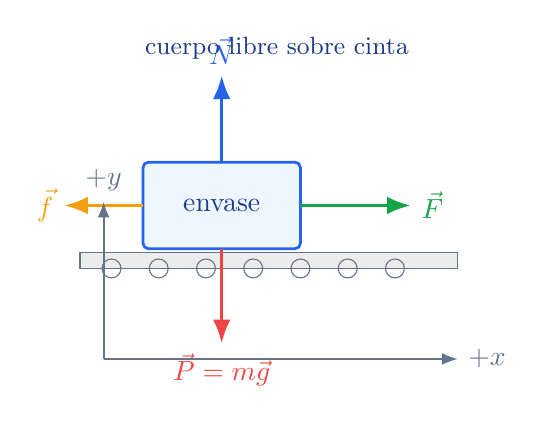
\begin{tikzpicture}[scale=1]
\draw[body] (1,.5) rectangle (3,1.6); \node[text=brand] at (2,1.05) {envase};
\draw[fill=gray!15, draw=muted] (.2,.25) rectangle (5,.45); \foreach \x in {.6,1.2,...,4.6}{\draw[muted] (\x,.25) circle (.12);}
\draw[force,color=brandtwo] (2,1.6)--(2,2.7) node[above] {$\vec N$};
\draw[force,color=accentred] (2,.5)--(2,-.7) node[below] {$\vec P=m\vec g$};
\draw[force,color=accentgreen] (3,1.05)--(4.4,1.05) node[right] {$\vec F$};
\draw[force,color=accentorange] (1,1.05)--(.0,1.05) node[left] {$\vec f$};
\draw[axis] (.5,-.9)--(5,-.9) node[right] {$+x$}; \draw[axis] (.5,-.9)--(.5,1.1) node[above] {$+y$};
\node[lab] at (2.7,3.05) {cuerpo libre sobre cinta};
\end{tikzpicture}

\end{document}